\begin{mdframed}[style=warning]
	\begin{ejercicio}
		\textbf{Conceptos: }
		\begin{enumerate}[a)]
			\item Interprete la ley de Faraday y la ley de Lenz.
		\end{enumerate}
	\end{ejercicio}
\end{mdframed}











\begin{mdframed}[style=warning]
	\begin{ejercicio}
		Un circuito plano tiene la forma de un triángulo isósceles, cuyos lados son dos barras fijas perpendiculares y una tercera barra $MN$  que se desplaza  perpendicularmente con velocidad constante $v$ como se indica en la figura. El circuito está colocado en un campo magnético uniforme $B$ que forma un ángulo $\alpha$ con la normal al plano del circuito. Sabiendo que la resistencia eléctrica de las barras por unidad de longitud es $r$, determine: 
		\begin{itemize}
			\item La potencia necesaria para desplazar la barra $MN$.
			\item La potencia disipada en calor en función de la posición de la barra.
		\end{itemize}
		\begin{figure}[H]
			\centering
			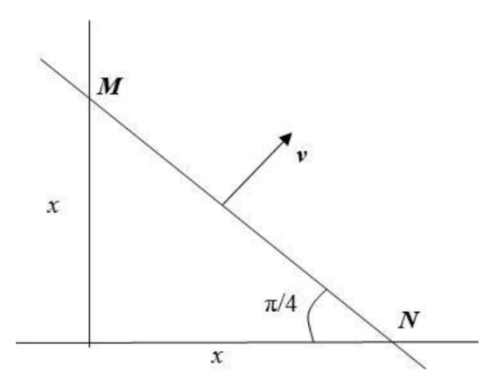
\includegraphics[scale=0.4]{./img/bar.png}
			\caption{Barra.}
			\label{espiras}	
		\end{figure}
	\end{ejercicio}
\end{mdframed}


















\begin{mdframed}[style=warning]
	\begin{ejercicio}
		En un alambre largo horizontal circula una corriente $I$ que decrece con el tiempo. Una espira conductora es suspendida durante un intervalo de tiempo $\Delta t$ pequeño. En ese intervalo la espira se mantiene en equilibrio. La espira se encuentra en un plano vertical a una distancia $D$ por debajo del alambre, como se muestra en la figura. La espira es un cuadrado de lado $a$, masa $m$ y resistencia $R$. La distancia $D$ es mucho mayor que $a$. Desprecie la autoinductancia de la espira.
		\begin{figure}[H]
			\centering
			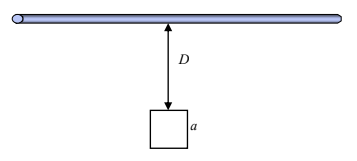
\includegraphics[scale=0.5]{./img/square.png}
			\caption{Levitación de una Espira Conductora.}
			\label{DF}	
		\end{figure}
		\begin{enumerate}[a)]
			\item Haga un diagrama del sistema indicando claramente las corrientes, campos magnéticos y fuerzas involucradas.
			\item Haciendo las aproximaciones que considere oportunas, encuentre la corriente inducida en la espira en función de $\flatfrac{\Delta I}{\Delta t}$.
			\item Encuentre la fuerza magnética sobre la espira, indicando su magnitud, dirección y sentido.
		\end{enumerate}
	\end{ejercicio}
\end{mdframed}
























\begin{mdframed}[style=warning]
	\begin{ejercicio}
		Una espira coplanar al plano $XZ$ tiene ancho $w$ y largo $l$. Existe un campo magnético en el espacio descrito por la siguiente función por partes
			$$
				\vec{B} = \left\{\begin{array}{cc}
					B_o \vy & z \leq 0 \\
					0 & z > 0.
				\end{array}\right.
			$$
		La espira esta también dentro de un campo gravitacional $\vec{g} = g_o \vz$ y tiene una masa $m_o$. Asimismo, su resistencia elécitrca tiene un valor de $R_o$. No existe ninguna fuente externa de alimentación de voltaje o corriente en el sistema. En $t = 0$ la bobina se suelta desde el reposo y su posición inicial en el eje de movimiento (medida desde la parte inferior de ésta) es $z(t = 0) = 0$. Para todas las preguntas asuma que $z(t) < l$, de tal forma que el alambre superior siempre se encuentre dentro de la región del campo magnético.
		\begin{figure}[H]
			\centering
			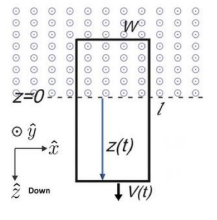
\includegraphics[scale=0.5]{./img/fall.png}
			\caption{Caída de Espira.}
			\label{DF}	
		\end{figure}
		\begin{enumerate}[a)]
			\item Determine la expresión para el flujo magnético $\Phi _B$ en la espira en términos de las variables y constantes conocidas. Su respuesta debe ser válida para todos los valores de $0 < z < l$. Escriba su respuesta en términos de $z$ y el resto de variables y constantes conocidas. La expresión NO debe depender del tiempo.
			\item Si luego de haber partido del reposo, la espira lleva una rapidez $v$, determine el vector de fuerza magnética neto que actúa sobre la espira para este valor de rapidez $v$. Escriba su respuesta en términos de las variables y constantes conocidas (incluida $v$).
			\item Determine una expresión para la magnitud de la velocidad terminal de caída de la espira. Se le llama velocidad terminal cuando se llega a una velocidad máxima y el objeto no acelera más. Escriba su respuesta en términos de las variables y constantes conocidas (incluida $v$). Recuerde, siempre se cumple que $z(t) < l$.
		\end{enumerate}
	\end{ejercicio}
\end{mdframed}




























































%%%%%


















































%%%